\documentclass[12pt,a4paper]{article}
\usepackage[utf8]{inputenc}
\usepackage[T1]{fontenc}
\usepackage{textcomp}
\usepackage{graphicx}
\usepackage{booktabs}
\usepackage{tabularx}
\usepackage{float}
\usepackage[margin=1in]{geometry}
\usepackage{url}
\usepackage{hyperref}
\hypersetup{hidelinks}
\graphicspath{{figures/}}

\title{CS 464 \\ Progress Report: Robust Room Occupancy Estimation \\ Group 20}
\author{Turan Emre Adıgüzel 22203033 \\ Ali Osman Karahasanoğlu 22201636 \\ Batıkan Bora Özüer 22202849 \\ Merve Topuz 22302937 \\ Öykü Kurt 22202131}
\date{November 29, 2026}

\begin{document}
\maketitle
\thispagestyle{empty}
\begin{center}
\includegraphics[width=0.6\textwidth]{bilkent_logo.png}\end{center}
\newpage
\setcounter{page}{1}
\tableofcontents
\newpage

\section{Introduction}
The goal of this project is to estimate the number of people in a room (0, 1, 2 or 3) from non-intrusive environmental sensors (temperature, light, sound, CO\textsubscript{2} and passive-infrared motion) instead of cameras. Camera-free occupancy estimation is useful for energy-efficient heating, ventilation and lighting control while preserving privacy.

We will also test how performance changes when sensors are removed, measurements become noisy, or readings are missing. The final study will compare Logistic Regression, Random Forest, XGBoost and a Multi-Layer Perceptron on the same day-based evaluation protocol.

This progress report covers the first phase: dataset analysis, the fixed train/validation/test split that all later experiments will share, and initial results of a Random Forest baseline. The baseline performs well on the test day (macro-F1 0.906) but much worse on the validation days; for example, class-3 F1 falls from 0.901 on 23 December 2017 to 0.063 on 10 January 2018.

\section{Dataset}
\subsection{Dataset Analysis}
We use the UCI Room Occupancy Estimation dataset [1, 2]: 10,129 tabular samples recorded every \textasciitilde{}30 seconds (median interval 31 s) in a room between 22 December 2017 and 11 January 2018. There are no missing values and no images; each sample has a date, a time, 16 numeric sensor features and the label \texttt{Room\_Occupancy\_Count}. The sensors are summarised in Table 1.

\begin{table}[H]
\centering
\begin{tabular}{lll}
\toprule
\textbf{Sensor type} & \textbf{Features} & \textbf{Unit / range} \\
\midrule
Temperature & S1--S4\_Temp & 24.4--29.0 \textdegree{}C \\
Light & S1--S4\_Light & 0--280 lux \\
Sound & S1--S4\_Sound & 0.04--3.88 V (microphone amplitude) \\
CO\textsubscript{2} & S5\_CO\textsubscript{2}, S5\_CO\textsubscript{2}\_Slope & 345--1270 ppm; slope over a sliding window \\
Motion (PIR) & S6\_PIR, S7\_PIR & binary 0/1 \\
\bottomrule
\end{tabular}
\caption{Sensor features in the dataset}
\end{table}

The target has four classes (0, 1, 2, 3 occupants) and is highly imbalanced: an empty room accounts for 81.2\% of the samples (Table 2).

\begin{table}[H]
\centering
\begin{tabular}{crr}
\toprule
\textbf{Occupants} & \textbf{Samples} & \textbf{Share} \\
\midrule
0 & 8,228 & 81.2\% \\
1 & 459 & 4.5\% \\
2 & 748 & 7.4\% \\
3 & 694 & 6.9\% \\
\bottomrule
\end{tabular}
\caption{Class distribution of the whole dataset}
\end{table}

Two findings from the analysis shape the rest of the project:

\begin{itemize}
  \item \textbf{Occupancy is concentrated in three days.} Only 22 Dec 2017, 23 Dec 2017 and 10 Jan 2018 contain people; the other four days contain only empty-room samples. Class 1 appears only on 22 and 23 Dec 2017.
  \item \textbf{Light, sound and CO\textsubscript{2} separate the classes most clearly.} Mean S1\_Light is 2.7 lux for an empty room versus 113--136 lux when occupied, and mean CO\textsubscript{2} rises from 404 ppm (0 people) to 851 ppm (3 people). Mean temperature differs by less than 1 \textdegree{}C between classes. The four light sensors are strongly correlated with each other, as are the four temperature sensors.
\end{itemize}

\begin{figure}[H]
\centering
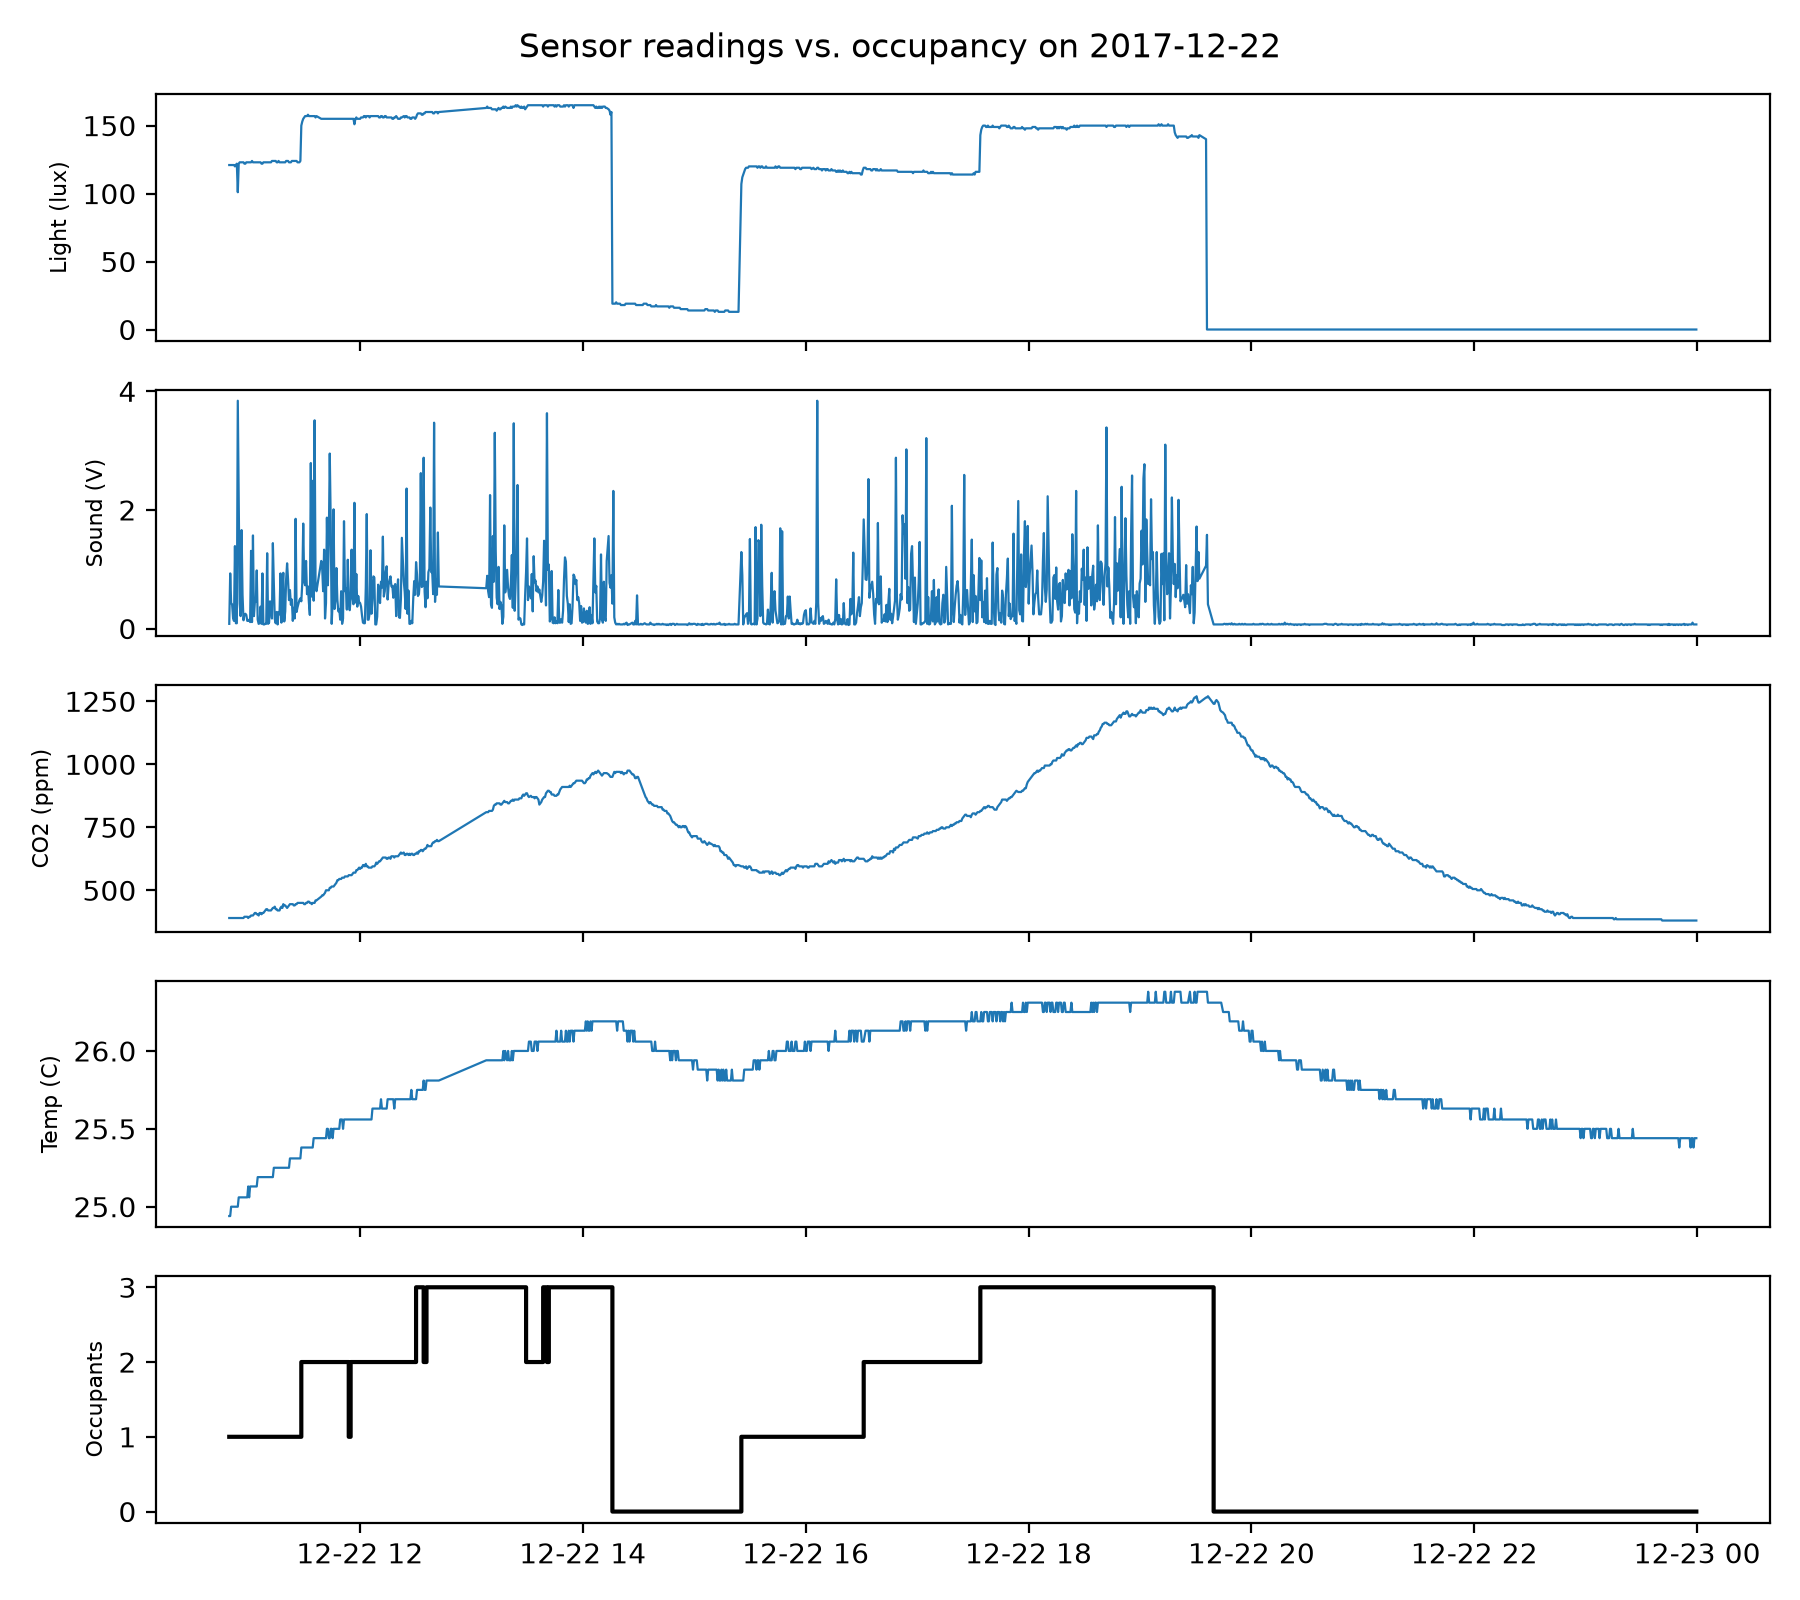
\includegraphics[width=0.80\textwidth]{timeseries_2017-12-22.png}
\caption{Light, sound, CO\textsubscript{2} and temperature on 22 Dec 2017 with the true occupant count (bottom). Light and sound change with occupancy almost instantly; CO\textsubscript{2} and temperature follow with a delay.}
\end{figure}

Figure 1 shows one occupied day. Figure 2 shows the distribution of six features per class: an empty room is clearly separated, while classes 2 and 3 overlap strongly.

\begin{figure}[H]
\centering
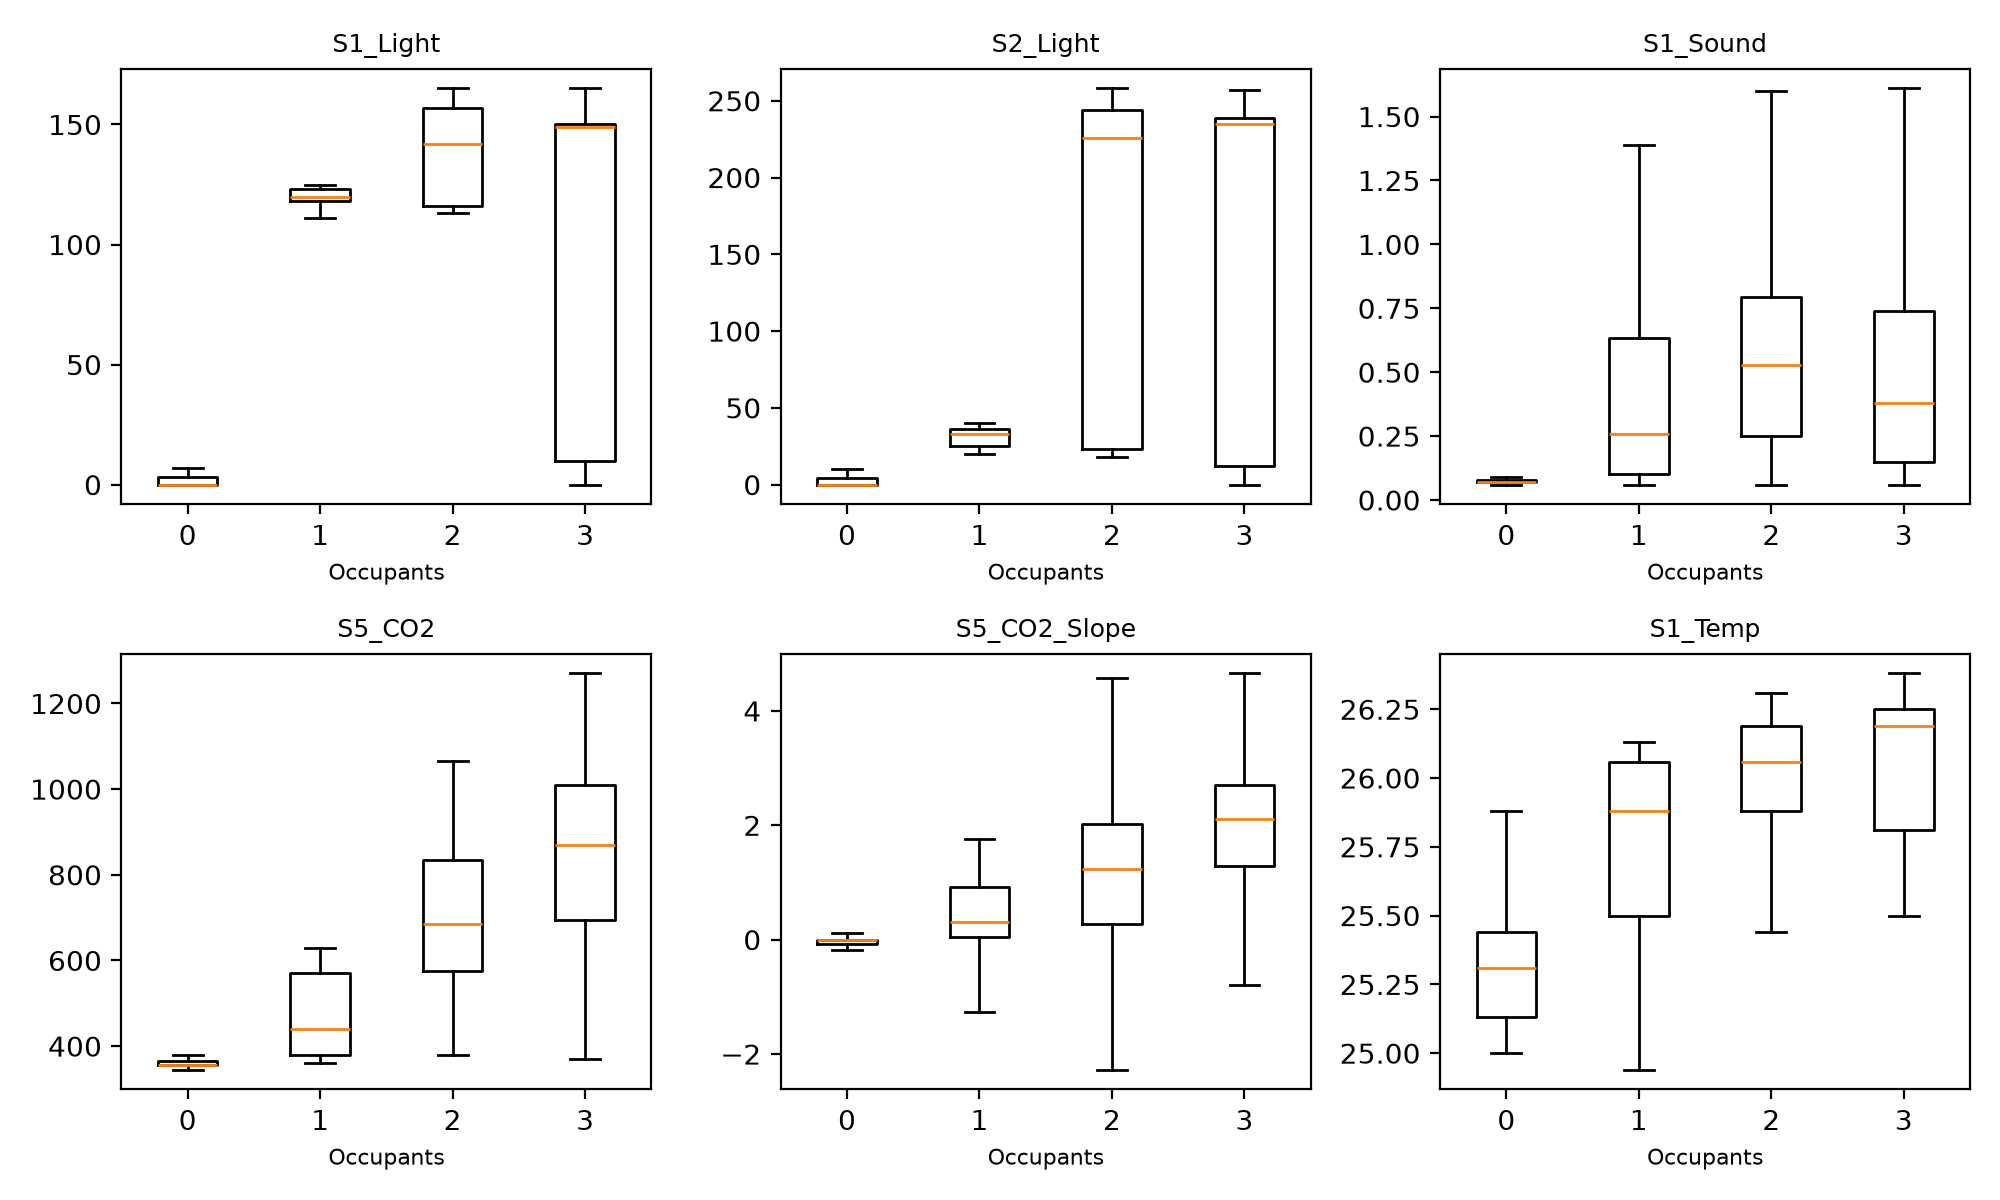
\includegraphics[width=0.90\textwidth]{feature_by_class.png}
\caption{Distribution of six features per class (box = interquartile range, outliers hidden).}
\end{figure}

\subsection{Dataset Preprocessing}
\textbf{Split.} Consecutive readings 30 s apart are nearly identical, so a random split puts near-duplicates of test samples into training and gives optimistic scores (Section 6.4). Following our TA's feedback, we use a \textbf{day-based split} in which validation days are separate from test days, and \textbf{the same split is used for every model and experiment} (defined once in the code). Because only three days are occupied, each split receives exactly one occupied day, plus empty days to balance sizes (Table 3, Figure 3).

\begin{table}[H]
\centering
\begin{tabular}{llrrrrr}
\toprule
\textbf{Split} & \textbf{Days} & \textbf{0} & \textbf{1} & \textbf{2} & \textbf{3} & \textbf{Total} \\
\midrule
Train & 22, 24, 25, 26 Dec 2017 & 4,480 & 205 & 257 & 363 & 5,305 (52\%) \\
Validation & 10, 11 Jan 2018 & 1,751 & 0 & 93 & 201 & 2,045 (20\%) \\
Test & 23 Dec 2017 & 1,997 & 254 & 398 & 130 & 2,779 (27\%) \\
\bottomrule
\end{tabular}
\caption{Fixed day-based split and samples per class}
\end{table}

\begin{figure}[H]
\centering
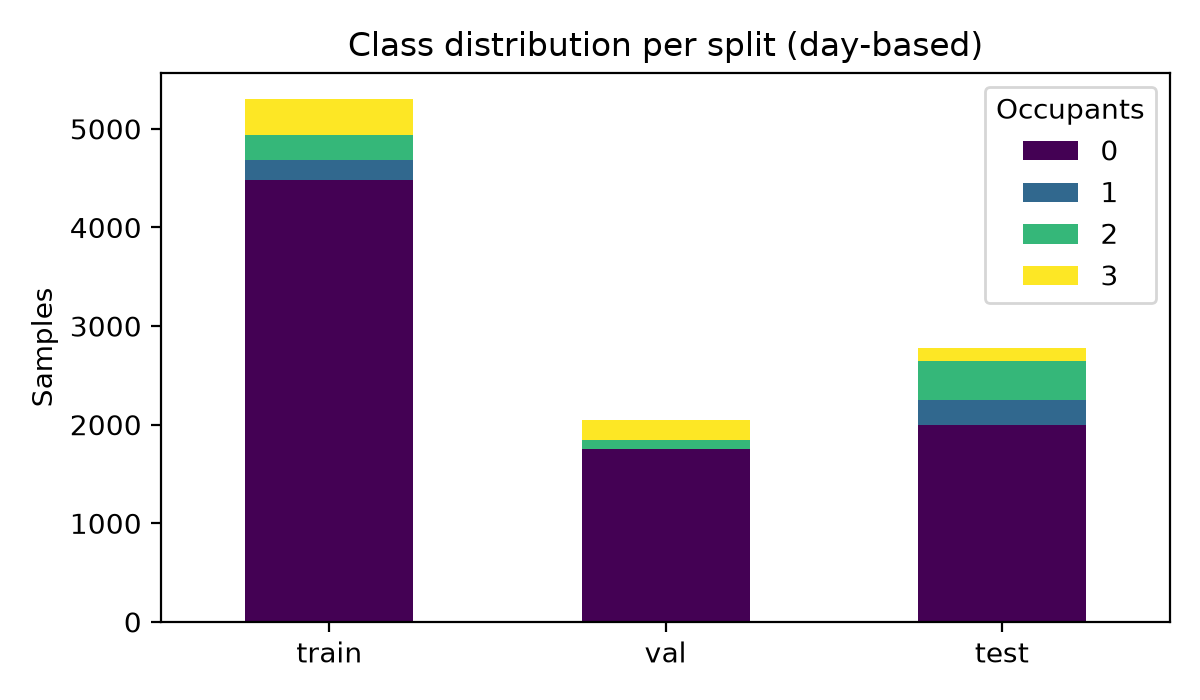
\includegraphics[width=0.60\textwidth]{split_distribution.png}
\caption{Class distribution per split.}
\end{figure}

Train and test contain all four classes. The validation days contain no class-1 samples: class 1 exists only on two days, so it cannot appear in three disjoint day groups. This is a structural limit of the dataset. Validation macro-F1 is therefore computed over a fixed label set \{0, 2, 3\} (\texttt{zero\_division = 0}), the same for every model, and class-1 performance cannot be monitored on validation during tuning. We plan to confirm this choice with our TA.

\textbf{Other steps.} Date and Time are dropped from the features so the model cannot memorise when a day was recorded. No imputation is needed. Tree-based models do not require feature scaling; for Logistic Regression and the MLP in the next phase, a standard scaler will be fitted on the training split only.

\section{Coding Environment}
All code is written in Python 3.12 and runs on a standard laptop CPU; Random Forest training takes about 0.5 s, so no GPU is needed at this stage. The tools are listed in Table 4.

\begin{table}[H]
\centering
\begin{tabular}{ll}
\toprule
\textbf{Tool} & \textbf{Use} \\
\midrule
pandas, NumPy & Loading the CSV, time stamps, split construction, statistics \\
scikit-learn 1.9 [4] & Random Forest, metrics (macro-F1, accuracy, confusion matrix) \\
Matplotlib [5] & All figures in this report \\
Git + GitHub & Version control and sharing within the team \\
XGBoost, PyTorch (planned) & XGBoost and MLP models in the next phase \\
\bottomrule
\end{tabular}
\caption{Tools and libraries}
\end{table}

The code is public on GitHub [6]. \texttt{src/common.py} holds data loading and the fixed split, \texttt{src/eda.py} produces the dataset analysis, and \texttt{src/train\_rf.py} trains and evaluates the baseline. All results can be reproduced by installing \texttt{requirements.txt} and running \texttt{python eda.py} and \texttt{python train\_rf.py} inside \texttt{src/}.

\section{Details of the Trained Model: Random Forest}
We chose \textbf{Random Forest} [3] as the first model because it needs no feature scaling, handles correlated features, trains in under a second on this data, and reports feature importances that feed directly into the planned sensor-ablation study.

\textbf{How it works.} A Random Forest is an ensemble of decision trees. Each tree is trained on a bootstrap sample of the training set (sampling with replacement), and at every split it only considers a random subset of the features. Each tree greedily chooses the feature and threshold that most reduce Gini impurity, 1 $-$ $\sum$ $p_k^2$, where $p_k$ is the fraction of class k in the node. At prediction time the trees' class probabilities are averaged and the most likely class is returned. Bootstrapping and feature subsampling make the trees less correlated, so averaging them reduces variance compared with a single deep tree.

\textbf{Hyperparameters and their expected effects.} The baseline uses scikit-learn defaults (Table 5); tuning on the validation split is planned for the final report. A fixed random seed (42) is used so that results are reproducible.

\begin{table}[H]
\centering
\begin{tabularx}{\textwidth}{llX}
\toprule
\textbf{Hyperparameter} & \textbf{Value} & \textbf{Expected effect} \\
\midrule
n\_estimators & 100 & More trees give more stable predictions with diminishing returns; training and inference time grow linearly. \\
max\_depth & None & Fully grown trees fit the training data perfectly (train macro-F1 = 1.0); limiting depth adds bias but can generalise better across days. \\
max\_features & sqrt(16) = 4 & Fewer features per split decorrelate the trees; more features make each tree stronger but the ensemble more similar. \\
min\_samples\_leaf & 1 & Larger leaves smooth the decision boundary and reduce overfitting to near-duplicate readings. \\
class\_weight & None & ''balanced'' re-weights classes by inverse frequency, which should help the minority classes 1--3. \\
criterion & gini & Entropy usually gives similar results; minor effect expected. \\
\bottomrule
\end{tabularx}
\caption{Random Forest hyperparameters of the baseline and their expected effects}
\end{table}

\section{Experimental Setup}
The baseline Random Forest is trained on the training days with all 16 sensor features and evaluated on the training, validation and test splits. A second Random Forest with identical settings is trained on a stratified random 80/20 split, only as a reference. Because 81\% of samples are empty-room readings, \textbf{macro-F1 is the main metric} (the unweighted mean of per-class F1, so each class counts equally); accuracy is reported as a secondary score. We also report per-class F1, a confusion matrix, feature importances and training/inference time.

The goals of this first set of experiments are:

\begin{enumerate}
  \item Establish a reproducible baseline on the fixed day-based split that every later model is compared against on the same test day.
  \item Show how optimistic a random split is compared with the day-based split (reference only, not used for model selection).
  \item Identify which sensors the model relies on, as input for the sensor-ablation experiment.
\end{enumerate}

The protocol for the rest of the project follows our TA's feedback. In this phase the test day was used only to report the untuned baseline. From now on, all model and hyperparameter choices will be made on the validation split, and the final comparison of all models will be done on the same test day with the same split.

\textbf{Planned experiments for the final report:} Logistic Regression, XGBoost and an MLP on the same split; hyperparameter tuning; sensor ablation (subsets of sensor types); noise robustness (Gaussian noise of increasing strength); missing-sensor simulation with different imputation strategies; class-imbalance handling (class weighting, resampling); and an efficiency comparison (inference time versus macro-F1).

\section{Results}
The Random Forest baseline reaches a test macro-F1 of \textbf{0.906} (accuracy 0.945) on the held-out test day. On the validation days it reaches 0.429; computed over the same three classes (0, 2, 3), the test score is 0.884, so the drop between days remains large. A random split gives 0.990 (Table 6). Training took 0.46 s and inference about 0.01 ms per sample.

\begin{table}[H]
\centering
\begin{tabular}{lrr}
\toprule
\textbf{Evaluation} & \textbf{Macro-F1} & \textbf{Accuracy} \\
\midrule
Train (22, 24--26 Dec 2017) & 1.000 & 1.000 \\
Validation (10--11 Jan 2018), classes 0/2/3 & 0.429 & 0.868 \\
Test (23 Dec 2017), classes 0/2/3 & 0.884 & -- \\
\textbf{Test (23 Dec 2017), all classes} & \textbf{0.906} & \textbf{0.945} \\
Random 80/20 split (reference) & 0.990 & 0.997 \\
\bottomrule
\end{tabular}
\caption{Random Forest baseline results}
\end{table}

\subsection{Test Day}
\begin{figure}[H]
\centering
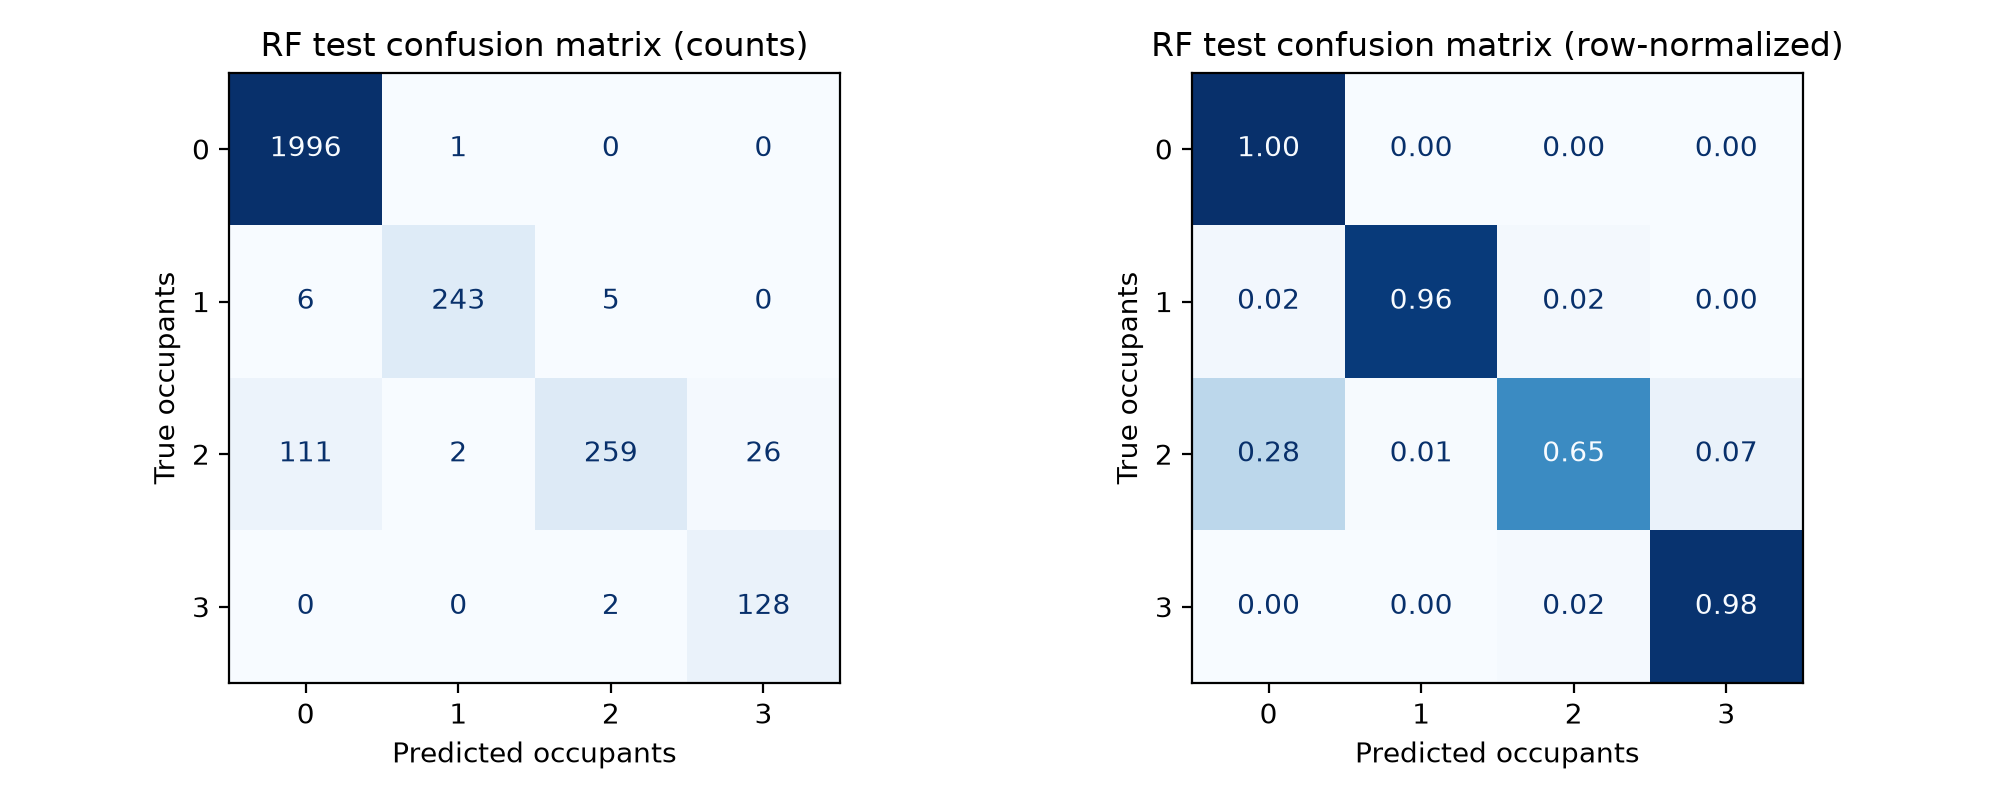
\includegraphics[width=0.95\textwidth]{rf_confusion_matrix.png}
\caption{Random Forest confusion matrix on the test day (23 Dec 2017): counts (left) and row-normalised (right).}
\end{figure}

The weakest class is 2 occupants: 111 of 398 samples (28\%) are predicted as an empty room, and 26 as three people (Figure 4). Classes 0, 1 and 3 are recognised with F1 at or above 0.90 (Table 7).

\begin{table}[H]
\centering
\begin{tabular}{lrrrr}
\toprule
\textbf{} & \textbf{Precision} & \textbf{Recall} & \textbf{F1-Score} & \textbf{Support} \\
\midrule
0 occupants & 0.94 & 1.00 & 0.97 & 1997 \\
1 occupant & 0.99 & 0.96 & 0.97 & 254 \\
2 occupants & 0.97 & 0.65 & 0.78 & 398 \\
3 occupants & 0.83 & 0.98 & 0.90 & 130 \\
\midrule
\textbf{Accuracy} &  &  & \textbf{0.94} & \textbf{2779} \\
\textbf{Macro Avg} & \textbf{0.93} & \textbf{0.90} & \textbf{0.91} & \textbf{2779} \\
\textbf{Weighted Avg} & \textbf{0.95} & \textbf{0.94} & \textbf{0.94} & \textbf{2779} \\
\bottomrule
\end{tabular}
\caption{Random Forest classification report on the test day}
\end{table}

\subsection{Feature Importance}
The model relies mostly on light: S2\_Light (0.208) and S1\_Light (0.205) together account for 41\% of the total Gini importance, followed by S5\_CO\textsubscript{2}\_Slope (0.115), S3\_Light (0.094) and S5\_CO\textsubscript{2} (0.077) (Figure 5). The two PIR motion sensors have very low Gini importance (0.002 and 0.001). Gini importance is affected by correlated features, so this does not show that PIR is useless; the sensor-ablation experiment will test whether it adds predictive value.

\begin{figure}[H]
\centering
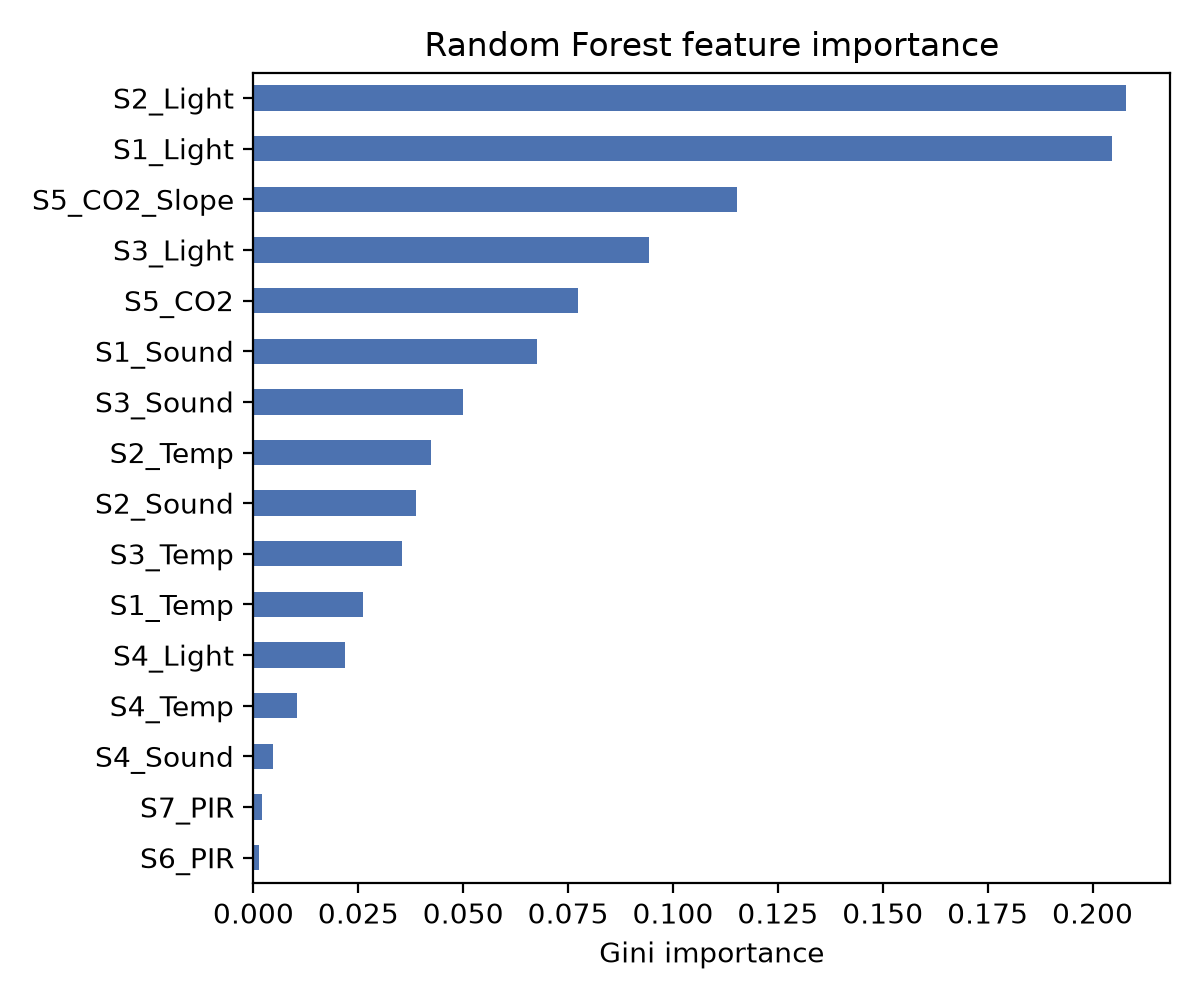
\includegraphics[width=0.60\textwidth]{rf_feature_importance.png}
\caption{Gini feature importance of the Random Forest baseline.}
\end{figure}

\subsection{Why Validation Is Much Lower: A Shift Between Days}
On 10 Jan 2018, with three people present, mean S1\_Light is 18 lux and S2\_Light 26 lux, compared with 150--240 lux for three people in December. The model labels 184 of 201 three-person samples as empty and reaches only 0.063 F1 for class 3. Other sensors still indicate presence: mean CO\textsubscript{2} is 554 ppm and the PIR sensors are active in 55\% and 68\% of these samples, compared with 0\% for the empty room. Why light was low that day is not known from the data.

The January results suggest that the baseline, which relies most on light, does not generalise well to occupied periods with low light levels. The sensor-ablation, noise and missing-sensor experiments will test whether reducing reliance on light improves validation performance; CO\textsubscript{2} and motion are candidates for this analysis.

\subsection{Random Versus Day-Based Split}
With a random split the same model scores 0.990 macro-F1. Near-duplicate readings 30 s apart fall on both sides of a random split; training size and day composition also differ, so the gap cannot be attributed to leakage alone. The day-based split keeps each day's readings in one partition and evaluates the model on a day excluded from training. The 74\% day-based macro-F1 in our proposal came from a different preliminary split and is not directly comparable to these results.

These results come from a single test day; they show how the baseline behaves on that day, not its general robustness.

\section{Division of Work Among Teammates}
We divided the workload as follows:

\begin{itemize}
  \item \textbf{Batıkan Bora Özüer}: Repository setup, data pipeline, day-based split, Random Forest baseline and progress report preparation.
  \item \textbf{Turan Emre Adıgüzel}: [to be filled]
  \item \textbf{Ali Osman Karahasanoğlu}: [to be filled]
  \item \textbf{Merve Topuz}: [to be filled]
  \item \textbf{Öykü Kurt}: [to be filled]
\end{itemize}

\begin{thebibliography}{9}
\bibitem{r1} A. P. Singh, V. Jain, S. Chaudhari, F. A. Kraemer, S. Werner and V. Garg, ''Machine Learning-Based Occupancy Estimation Using Multivariate Sensor Nodes,'' in \textit{2018 IEEE Globecom Workshops (GC Wkshps)}, Abu Dhabi, 2018.
\bibitem{r2} A. P. Singh and S. Chaudhari, \textit{Room Occupancy Estimation} [Dataset], UCI Machine Learning Repository, 2018. DOI: 10.24432/C5P605. Available: \url{https://archive.ics.uci.edu/dataset/864/room+occupancy+estimation}.
\bibitem{r3} L. Breiman, ''Random Forests,'' \textit{Machine Learning}, vol. 45, no. 1, pp. 5--32, 2001.
\bibitem{r4} F. Pedregosa et al., ''Scikit-learn: Machine Learning in Python,'' \textit{Journal of Machine Learning Research}, vol. 12, pp. 2825--2830, 2011.
\bibitem{r5} J. D. Hunter, ''Matplotlib: A 2D Graphics Environment,'' \textit{Computing in Science \& Engineering}, vol. 9, no. 3, pp. 90--95, 2007.
\bibitem{r6} Project repository, \textit{CS464-Room-Occupancy}, GitHub. Available: \url{https://github.com/batikanborao-cmd/CS464-Room-Occupancy}.
\end{thebibliography}
\end{document}
